% Created by tikzDevice version 0.10.1 on 2020-02-15 16:13:19
% !TEX encoding = UTF-8 Unicode
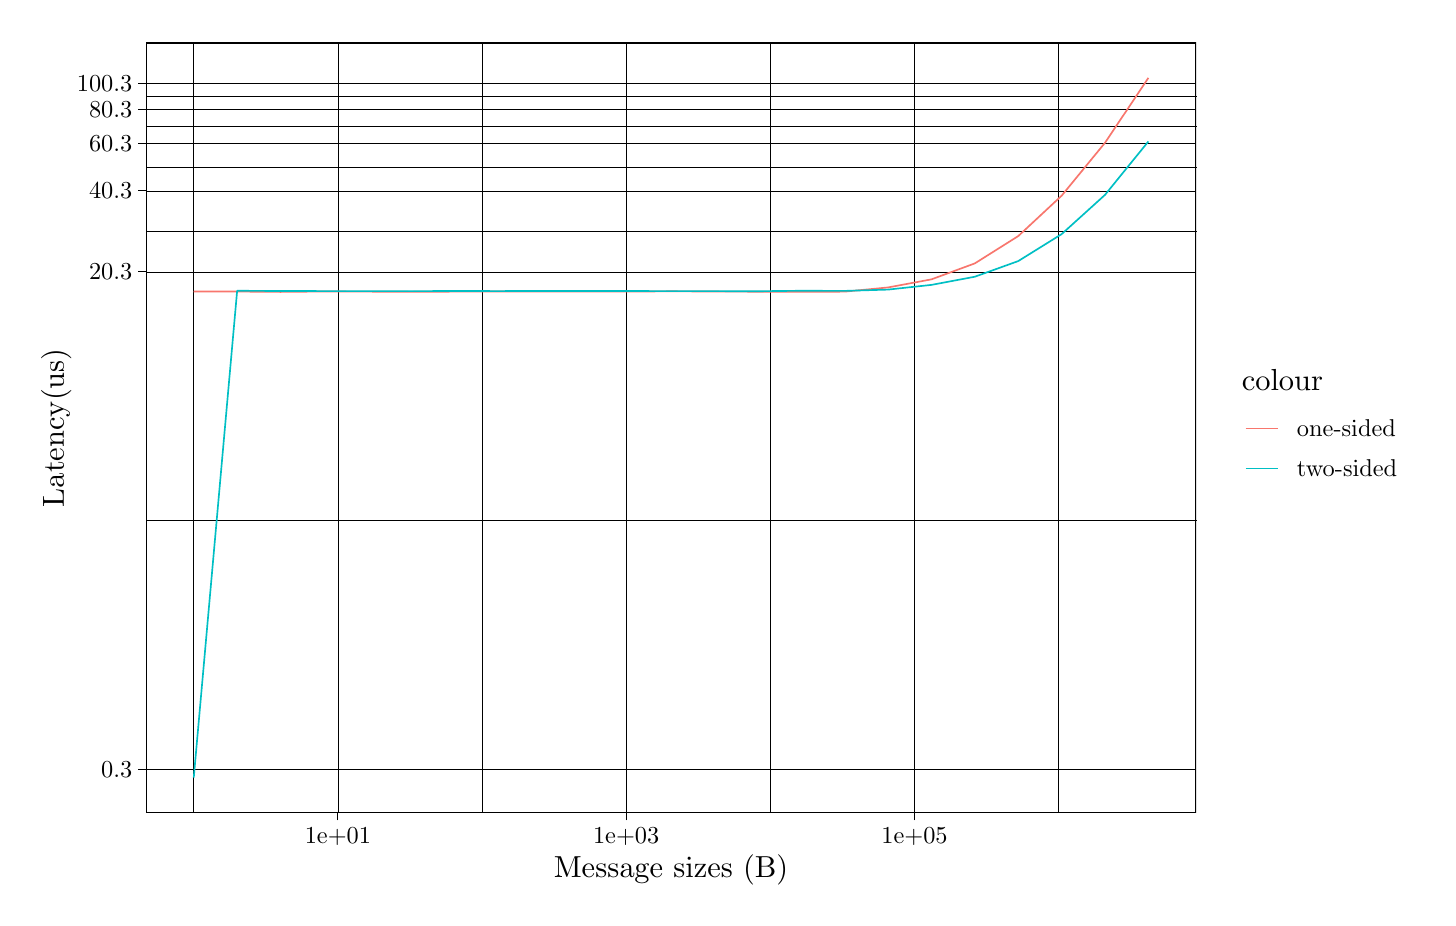
\begin{tikzpicture}[x=1pt,y=1pt]
\definecolor{fillColor}{RGB}{255,255,255}
\path[use as bounding box,fill=fillColor,fill opacity=0.00] (0,0) rectangle (505.89,314.37);
\begin{scope}
\path[clip] (  0.00,  0.00) rectangle (505.89,314.37);
\definecolor{drawColor}{RGB}{255,255,255}
\definecolor{fillColor}{RGB}{255,255,255}

\path[draw=drawColor,line width= 0.6pt,line join=round,line cap=round,fill=fillColor] (  0.00,  0.00) rectangle (505.89,314.37);
\end{scope}
\begin{scope}
\path[clip] ( 42.76, 30.72) rectangle (422.22,308.87);
\definecolor{fillColor}{RGB}{255,255,255}

\path[fill=fillColor] ( 42.76, 30.72) rectangle (422.22,308.87);
\definecolor{drawColor}{RGB}{0,0,0}

\path[draw=drawColor,line width= 0.0pt,line join=round] ( 42.76,136.22) --
	(422.22,136.22);

\path[draw=drawColor,line width= 0.0pt,line join=round] ( 42.76,240.75) --
	(422.22,240.75);

\path[draw=drawColor,line width= 0.0pt,line join=round] ( 42.76,263.98) --
	(422.22,263.98);

\path[draw=drawColor,line width= 0.0pt,line join=round] ( 42.76,278.69) --
	(422.22,278.69);

\path[draw=drawColor,line width= 0.0pt,line join=round] ( 42.76,289.54) --
	(422.22,289.54);

\path[draw=drawColor,line width= 0.0pt,line join=round] ( 60.01, 30.72) --
	( 60.01,308.87);

\path[draw=drawColor,line width= 0.0pt,line join=round] (164.18, 30.72) --
	(164.18,308.87);

\path[draw=drawColor,line width= 0.0pt,line join=round] (268.36, 30.72) --
	(268.36,308.87);

\path[draw=drawColor,line width= 0.0pt,line join=round] (372.54, 30.72) --
	(372.54,308.87);

\path[draw=drawColor,line width= 0.1pt,line join=round] ( 42.76, 46.31) --
	(422.22, 46.31);

\path[draw=drawColor,line width= 0.1pt,line join=round] ( 42.76,226.13) --
	(422.22,226.13);

\path[draw=drawColor,line width= 0.1pt,line join=round] ( 42.76,255.38) --
	(422.22,255.38);

\path[draw=drawColor,line width= 0.1pt,line join=round] ( 42.76,272.58) --
	(422.22,272.58);

\path[draw=drawColor,line width= 0.1pt,line join=round] ( 42.76,284.80) --
	(422.22,284.80);

\path[draw=drawColor,line width= 0.1pt,line join=round] ( 42.76,294.29) --
	(422.22,294.29);

\path[draw=drawColor,line width= 0.1pt,line join=round] (112.10, 30.72) --
	(112.10,308.87);

\path[draw=drawColor,line width= 0.1pt,line join=round] (216.27, 30.72) --
	(216.27,308.87);

\path[draw=drawColor,line width= 0.1pt,line join=round] (320.45, 30.72) --
	(320.45,308.87);
\definecolor{drawColor}{RGB}{248,118,109}

\path[draw=drawColor,line width= 0.6pt,line join=round] ( 60.01,219.06) --
	( 75.69,219.01) --
	( 91.37,218.88) --
	(107.05,219.03) --
	(122.73,218.98) --
	(138.41,218.91) --
	(154.09,218.98) --
	(169.77,219.01) --
	(185.45,219.03) --
	(201.13,219.06) --
	(216.81,218.98) --
	(232.49,219.11) --
	(248.17,219.01) --
	(263.85,218.96) --
	(279.53,218.91) --
	(295.21,218.98) --
	(310.89,220.50) --
	(326.57,223.42) --
	(342.25,229.19) --
	(357.93,239.05) --
	(373.61,253.64) --
	(389.29,272.77) --
	(404.97,296.23);
\definecolor{drawColor}{RGB}{0,191,196}

\path[draw=drawColor,line width= 0.6pt,line join=round] ( 60.01, 43.37) --
	( 75.69,219.30) --
	( 91.37,219.21) --
	(107.05,219.18) --
	(122.73,219.16) --
	(138.41,219.16) --
	(154.09,219.21) --
	(169.77,219.18) --
	(185.45,219.21) --
	(201.13,219.21) --
	(216.81,219.21) --
	(232.49,219.16) --
	(248.17,219.16) --
	(263.85,219.13) --
	(279.53,219.30) --
	(295.21,219.25) --
	(310.89,219.72) --
	(326.57,221.42) --
	(342.25,224.37) --
	(357.93,230.02) --
	(373.61,239.76) --
	(389.29,253.95) --
	(404.97,273.26);
\definecolor{drawColor}{RGB}{0,0,0}

\path[draw=drawColor,line width= 0.6pt,line join=round,line cap=round] ( 42.76, 30.72) rectangle (422.22,308.87);
\end{scope}
\begin{scope}
\path[clip] (  0.00,  0.00) rectangle (505.89,314.37);
\definecolor{drawColor}{RGB}{0,0,0}

\node[text=drawColor,anchor=base west,inner sep=0pt, outer sep=0pt, scale=  0.88] at ( 26.57, 43.49) {0.3};

\node[text=drawColor,anchor=base west,inner sep=0pt, outer sep=0pt, scale=  0.88] at ( 22.17,223.30) {20.3};

\node[text=drawColor,anchor=base west,inner sep=0pt, outer sep=0pt, scale=  0.88] at ( 22.17,252.56) {40.3};

\node[text=drawColor,anchor=base west,inner sep=0pt, outer sep=0pt, scale=  0.88] at ( 22.17,269.75) {60.3};

\node[text=drawColor,anchor=base west,inner sep=0pt, outer sep=0pt, scale=  0.88] at ( 22.17,281.97) {80.3};

\node[text=drawColor,anchor=base west,inner sep=0pt, outer sep=0pt, scale=  0.88] at ( 17.77,291.46) {100.3};
\end{scope}
\begin{scope}
\path[clip] (  0.00,  0.00) rectangle (505.89,314.37);
\definecolor{drawColor}{RGB}{0,0,0}

\path[draw=drawColor,line width= 0.3pt,line join=round] ( 40.01, 46.31) --
	( 42.76, 46.31);

\path[draw=drawColor,line width= 0.3pt,line join=round] ( 40.01,226.13) --
	( 42.76,226.13);

\path[draw=drawColor,line width= 0.3pt,line join=round] ( 40.01,255.38) --
	( 42.76,255.38);

\path[draw=drawColor,line width= 0.3pt,line join=round] ( 40.01,272.58) --
	( 42.76,272.58);

\path[draw=drawColor,line width= 0.3pt,line join=round] ( 40.01,284.80) --
	( 42.76,284.80);

\path[draw=drawColor,line width= 0.3pt,line join=round] ( 40.01,294.29) --
	( 42.76,294.29);
\end{scope}
\begin{scope}
\path[clip] (  0.00,  0.00) rectangle (505.89,314.37);
\definecolor{drawColor}{RGB}{0,0,0}

\path[draw=drawColor,line width= 0.3pt,line join=round] (112.10, 27.97) --
	(112.10, 30.72);

\path[draw=drawColor,line width= 0.3pt,line join=round] (216.27, 27.97) --
	(216.27, 30.72);

\path[draw=drawColor,line width= 0.3pt,line join=round] (320.45, 27.97) --
	(320.45, 30.72);
\end{scope}
\begin{scope}
\path[clip] (  0.00,  0.00) rectangle (505.89,314.37);
\definecolor{drawColor}{RGB}{0,0,0}

\node[text=drawColor,anchor=base,inner sep=0pt, outer sep=0pt, scale=  0.88] at (112.10, 19.71) {1e+01};

\node[text=drawColor,anchor=base,inner sep=0pt, outer sep=0pt, scale=  0.88] at (216.27, 19.71) {1e+03};

\node[text=drawColor,anchor=base,inner sep=0pt, outer sep=0pt, scale=  0.88] at (320.45, 19.71) {1e+05};
\end{scope}
\begin{scope}
\path[clip] (  0.00,  0.00) rectangle (505.89,314.37);
\definecolor{drawColor}{RGB}{0,0,0}

\node[text=drawColor,anchor=base,inner sep=0pt, outer sep=0pt, scale=  1.10] at (232.49,  7.44) {Message sizes (B)};
\end{scope}
\begin{scope}
\path[clip] (  0.00,  0.00) rectangle (505.89,314.37);
\definecolor{drawColor}{RGB}{0,0,0}

\node[text=drawColor,rotate= 90.00,anchor=base,inner sep=0pt, outer sep=0pt, scale=  1.10] at ( 13.08,169.80) {Latency(us)};
\end{scope}
\begin{scope}
\path[clip] (  0.00,  0.00) rectangle (505.89,314.37);
\definecolor{fillColor}{RGB}{255,255,255}

\path[fill=fillColor] (433.22,142.34) rectangle (500.39,197.26);
\end{scope}
\begin{scope}
\path[clip] (  0.00,  0.00) rectangle (505.89,314.37);
\definecolor{drawColor}{RGB}{0,0,0}

\node[text=drawColor,anchor=base west,inner sep=0pt, outer sep=0pt, scale=  1.10] at (438.72,183.22) {colour};
\end{scope}
\begin{scope}
\path[clip] (  0.00,  0.00) rectangle (505.89,314.37);
\definecolor{fillColor}{RGB}{255,255,255}

\path[fill=fillColor] (438.72,162.29) rectangle (453.17,176.74);
\end{scope}
\begin{scope}
\path[clip] (  0.00,  0.00) rectangle (505.89,314.37);
\definecolor{drawColor}{RGB}{248,118,109}

\path[draw=drawColor,line width= 0.6pt,line join=round] (440.16,169.52) -- (451.73,169.52);
\end{scope}
\begin{scope}
\path[clip] (  0.00,  0.00) rectangle (505.89,314.37);
\definecolor{drawColor}{RGB}{248,118,109}

\path[draw=drawColor,line width= 0.6pt,line join=round] (440.16,169.52) -- (451.73,169.52);
\end{scope}
\begin{scope}
\path[clip] (  0.00,  0.00) rectangle (505.89,314.37);
\definecolor{fillColor}{RGB}{255,255,255}

\path[fill=fillColor] (438.72,147.84) rectangle (453.17,162.29);
\end{scope}
\begin{scope}
\path[clip] (  0.00,  0.00) rectangle (505.89,314.37);
\definecolor{drawColor}{RGB}{0,191,196}

\path[draw=drawColor,line width= 0.6pt,line join=round] (440.16,155.06) -- (451.73,155.06);
\end{scope}
\begin{scope}
\path[clip] (  0.00,  0.00) rectangle (505.89,314.37);
\definecolor{drawColor}{RGB}{0,191,196}

\path[draw=drawColor,line width= 0.6pt,line join=round] (440.16,155.06) -- (451.73,155.06);
\end{scope}
\begin{scope}
\path[clip] (  0.00,  0.00) rectangle (505.89,314.37);
\definecolor{drawColor}{RGB}{0,0,0}

\node[text=drawColor,anchor=base west,inner sep=0pt, outer sep=0pt, scale=  0.88] at (458.67,166.49) {one-sided};
\end{scope}
\begin{scope}
\path[clip] (  0.00,  0.00) rectangle (505.89,314.37);
\definecolor{drawColor}{RGB}{0,0,0}

\node[text=drawColor,anchor=base west,inner sep=0pt, outer sep=0pt, scale=  0.88] at (458.67,152.03) {two-sided};
\end{scope}
\end{tikzpicture}
